%\documentclass[12pt]{FSUBeamer_light}
\documentclass[12pt]{FSUBeamer_official}
\usepackage[ngerman]{babel}
\usepackage[utf8]{inputenc}
\usepackage{default}

\usepackage{layouts}
\usepackage[sfdefault]{roboto} % official font of FSU Jena

\usepackage{media9}


%TIKZ
\usepackage{pgf}
\usepackage{tikz}
\usepackage{circuitikz}

\usetikzlibrary{shapes,arrows}

\usepackage{mfirstuc}
\usepackage{glossaries}

\usetikzlibrary{arrows,automata}
\usetikzlibrary{positioning}
\tikzset{
	state/.style={rectangle,rounded corners,draw=black, very thick,minimum height=2em,inner sep=2pt,text centered,},
}

\usepackage{subcaption}

\usepackage[]{ragged2e}
\usepackage[]{blindtext}

\usepackage{smartdiagram}
%%topdown arrow smartdiagram
\makeatletter
\NewDocumentCommand{\smartdiagramx}{r[] m}{%
	\StrCut{#1}{:}\diagramtype\option
	\IfStrEq{\diagramtype}{priority descriptive diagram}{% true-priority descriptive diagram
		\pgfmathparse{subtract(\sm@core@priorityarrowwidth,\sm@core@priorityarrowheadextend)}
		\pgfmathsetmacro\sm@core@priorityticksize{\pgfmathresult/2}
		\pgfmathsetmacro\arrowtickxshift{(\sm@core@priorityarrowwidth-\sm@core@priorityticksize)/2}
		\begin{tikzpicture}[every node/.style={align=center,let hypenation}]
		\foreach \smitem [count=\xi] in {#2}{\global\let\maxsmitem\xi}
		\foreach \smitem [count=\xi] in {#2}{%
			\edef\col{\@nameuse{color@\xi}}
			\node[description,drop shadow](module\xi)
			at (0,0+\xi*\sm@core@descriptiveitemsysep) {\smitem};
			\draw[line width=\sm@core@prioritytick,\col]
			([xshift=-\arrowtickxshift pt]module\xi.base west)--
			($([xshift=-\arrowtickxshift pt]module\xi.base west)-(\sm@core@priorityticksize pt,0)$);
		}%
		\coordinate (A) at (module1);
		\coordinate (B) at (module\maxsmitem);
		\CalcHeight(A,B){heightmodules}
		\pgfmathadd{\heightmodules}{\sm@core@priorityarrowheightadvance}
		\pgfmathsetmacro{\distancemodules}{\pgfmathresult}
		\pgfmathsetmacro\arrowxshift{\sm@core@priorityarrowwidth/2}
		\begin{pgfonlayer}{background}
		\node[priority arrow,rotate=180,transform shape] at ([xshift=-\arrowxshift pt]module\maxsmitem.north west){};
		\end{pgfonlayer}
		\end{tikzpicture}
	}{}% end-priority descriptive diagram
}%

\pgfkeys{/pgf/.cd,
	parallelepiped offset x/.initial=2mm,
	parallelepiped offset y/.initial=2mm
}

\usetikzlibrary{positioning}

\pgfdeclareshape{parallelepiped}
{
	\inheritsavedanchors[from=rectangle] % this is nearly a rectangle
	\inheritanchorborder[from=rectangle]
	\inheritanchor[from=rectangle]{north}
	\inheritanchor[from=rectangle]{north west}
	\inheritanchor[from=rectangle]{north east}
	\inheritanchor[from=rectangle]{center}
	\inheritanchor[from=rectangle]{west}
	\inheritanchor[from=rectangle]{east}
	\inheritanchor[from=rectangle]{mid}
	\inheritanchor[from=rectangle]{mid west}
	\inheritanchor[from=rectangle]{mid east}
	\inheritanchor[from=rectangle]{base}
	\inheritanchor[from=rectangle]{base west}
	\inheritanchor[from=rectangle]{base east}
	\inheritanchor[from=rectangle]{south}
	\inheritanchor[from=rectangle]{south west}
	\inheritanchor[from=rectangle]{south east}
	\backgroundpath{
		% store lower right in xa/ya and upper right in xb/yb
		\southwest \pgf@xa=\pgf@x \pgf@ya=\pgf@y
		\northeast \pgf@xb=\pgf@x \pgf@yb=\pgf@y
		\pgfmathsetlength\pgfutil@tempdima{\pgfkeysvalueof{/pgf/parallelepiped
				offset x}}
		\pgfmathsetlength\pgfutil@tempdimb{\pgfkeysvalueof{/pgf/parallelepiped
				offset y}}
		\def\ppd@offset{\pgfpoint{\pgfutil@tempdima}{\pgfutil@tempdimb}}
		\pgfpathmoveto{\pgfqpoint{\pgf@xa}{\pgf@ya}}
		\pgfpathlineto{\pgfqpoint{\pgf@xb}{\pgf@ya}}
		\pgfpathlineto{\pgfqpoint{\pgf@xb}{\pgf@yb}}
		\pgfpathlineto{\pgfqpoint{\pgf@xa}{\pgf@yb}}
		\pgfpathclose
		\pgfpathmoveto{\pgfqpoint{\pgf@xb}{\pgf@ya}}
		\pgfpathlineto{\pgfpointadd{\pgfpoint{\pgf@xb}{\pgf@ya}}{\ppd@offset}}
		\pgfpathlineto{\pgfpointadd{\pgfpoint{\pgf@xb}{\pgf@yb}}{\ppd@offset}}
		\pgfpathlineto{\pgfpointadd{\pgfpoint{\pgf@xa}{\pgf@yb}}{\ppd@offset}}
		\pgfpathlineto{\pgfqpoint{\pgf@xa}{\pgf@yb}}
		\pgfpathmoveto{\pgfqpoint{\pgf@xb}{\pgf@yb}}
		\pgfpathlineto{\pgfpointadd{\pgfpoint{\pgf@xb}{\pgf@yb}}{\ppd@offset}}
	}
}
\makeatother

\tikzset{l3 switch/.style={
		parallelepiped,fill=switch, draw=white,
		minimum width=0.75cm,
		minimum height=0.75cm,
		parallelepiped offset x=1.75mm,
		parallelepiped offset y=1.25mm,
		path picture={
			\node[fill=white,
			circle,
			minimum size=6pt,
			inner sep=0pt,
			append after command={
				\pgfextra{
					\foreach \angle in {0,45,...,360}
					\draw[-latex,fill=white] (\tikzlastnode.\angle)--++(\angle:2.25mm);
				}
			}
			] 
			at ([xshift=-0.75mm,yshift=-0.5mm]path picture bounding box.center){};
		}
	},
	ports/.style={
		line width=0.3pt,
		top color=gray!20,
		bottom color=gray!80
	},
	rack switch/.style={
		parallelepiped,fill=white, draw,
		minimum width=1.25cm,
		minimum height=0.25cm,
		parallelepiped offset x=2mm,
		parallelepiped offset y=1.25mm,
		xscale=-1,
		path picture={
			\draw[top color=gray!5,bottom color=gray!40]
			(path picture bounding box.south west) rectangle 
			(path picture bounding box.north east);
			\coordinate (A-west) at ([xshift=-0.2cm]path picture bounding box.west);
			\coordinate (A-center) at ($(path picture bounding box.center)!0!(path
			picture bounding box.south)$);
			\foreach \x in {0.275,0.525,0.775}{
				\draw[ports]([yshift=-0.05cm]$(A-west)!\x!(A-center)$)
				rectangle +(0.1,0.05);
				\draw[ports]([yshift=-0.125cm]$(A-west)!\x!(A-center)$)
				rectangle +(0.1,0.05);
			} 
			\coordinate (A-east) at (path picture bounding box.east);
			\foreach \x in {0.085,0.21,0.335,0.455,0.635,0.755,0.875,1}{
				\draw[ports]([yshift=-0.1125cm]$(A-east)!\x!(A-center)$)
				rectangle +(0.05,0.1);       
			}
		}
	},
	server/.style={
		parallelepiped,
		fill=white, draw,
		minimum width=0.35cm,
		minimum height=0.75cm,
		parallelepiped offset x=3mm,
		parallelepiped offset y=2mm,
		xscale=-1,
		path picture={
			\draw[top color=gray!5,bottom color=gray!40]
			(path picture bounding box.south west) rectangle 
			(path picture bounding box.north east);
			\coordinate (A-center) at ($(path picture bounding box.center)!0!(path
			picture bounding box.south)$);
			\coordinate (A-west) at ([xshift=-0.575cm]path picture bounding box.west);
			\draw[ports]([yshift=0.1cm]$(A-west)!0!(A-center)$)
			rectangle +(0.2,0.065);
			\draw[ports]([yshift=0.01cm]$(A-west)!0.085!(A-center)$)
			rectangle +(0.15,0.05);
			\fill[black]([yshift=-0.35cm]$(A-west)!-0.1!(A-center)$)
			rectangle +(0.235,0.0175);
			\fill[black]([yshift=-0.385cm]$(A-west)!-0.1!(A-center)$)
			rectangle +(0.235,0.0175);
			\fill[black]([yshift=-0.42cm]$(A-west)!-0.1!(A-center)$)
			rectangle +(0.235,0.0175);
		}  
	},
}

\usetikzlibrary{calc, shadings, shadows, shapes.arrows}

% Styles for interfaces and edge labels
\tikzset{%
	interface/.style={draw, rectangle, rounded corners, font=\LARGE\sffamily},
	ethernet/.style={interface, fill=yellow!50},% ethernet interface
	serial/.style={interface, fill=green!70},% serial interface
	speed/.style={sloped, anchor=south, font=\large\sffamily},% line speed at edge
	route/.style={draw, shape=single arrow, single arrow head extend=4mm,
		minimum height=1.7cm, minimum width=3mm, white, fill=switch!20,
		drop shadow={opacity=.8, fill=switch}, font=\tiny}% inroute/outroute arrows
}
\newcommand*{\shift}{1.3cm}% For placing the arrows later

% The router icon
\newcommand*{\router}[1]{
	\begin{tikzpicture}    
	\coordinate (ll) at (-3,0.5);
	\coordinate (lr) at (3,0.5);
	\coordinate (ul) at (-3,2);
	\coordinate (ur) at (3,2);
	\shade [shading angle=90, left color=switch, right color=white] (ll)
	arc (-180:-60:3cm and .75cm) -- +(0,1.5) arc (-60:-180:3cm and .75cm)
	-- cycle;
	\shade [shading angle=270, right color=switch, left color=white!50] (lr)
	arc (0:-60:3cm and .75cm) -- +(0,1.5) arc (-60:0:3cm and .75cm) -- cycle;
	\draw [thick] (ll) arc (-180:0:3cm and .75cm)
	-- (ur) arc (0:-180:3cm and .75cm) -- cycle;
	\draw [thick, shade, upper left=switch, lower left=switch,
	upper right=switch, lower right=white] (ul)
	arc (-180:180:3cm and .75cm);
	\node at (0,0.5){\color{blue!60!black}\Huge #1};% The name of the router
	% The four arrows, symbols for incoming and outgoing routes:
	\begin{scope}[yshift=2cm, yscale=0.28, transform shape]
	\node[route, rotate=45, xshift=\shift] {\strut};
	\node[route, rotate=-45, xshift=-\shift] {\strut};
	\node[route, rotate=-135, xshift=\shift] {\strut};
	\node[route, rotate=135, xshift=-\shift] {\strut};
	\end{scope}
	\end{tikzpicture}}

\makeatletter
\pgfdeclareradialshading[tikz@ball]{cloud}{\pgfpoint{-0.275cm}{0.4cm}}{%
	color(0cm)=(tikz@ball!75!white);
	color(0.1cm)=(tikz@ball!85!white); 
	color(0.2cm)=(tikz@ball!95!white); 
	color(0.7cm)=(tikz@ball!89!black); 
	color(1cm)=(tikz@ball!75!black)
}
\tikzoption{cloud color}{\pgfutil@colorlet{tikz@ball}{#1}%
	\def\tikz@shading{cloud}\tikz@addmode{\tikz@mode@shadetrue}}
\makeatother

\tikzset{my cloud/.style={
		cloud, draw, aspect=2,
		cloud color={gray!5!white}
	}
}

\makeatother

%%gl�ttet die Schrift
\usepackage{ae}

\title[Music Similarity Analysis]{Music Similarity Analysis}
\subtitle{Using the Big Data Framework Spark}
\author[Schoder, Johannes]{Johannes Schoder}
\institute[FSU Jena]{Fakultät für Mathematik und Informatik\\
	Friedrich-Schiller-Universität Jena}
\date[WiSe 2019]{\today}
%\titlegraphic{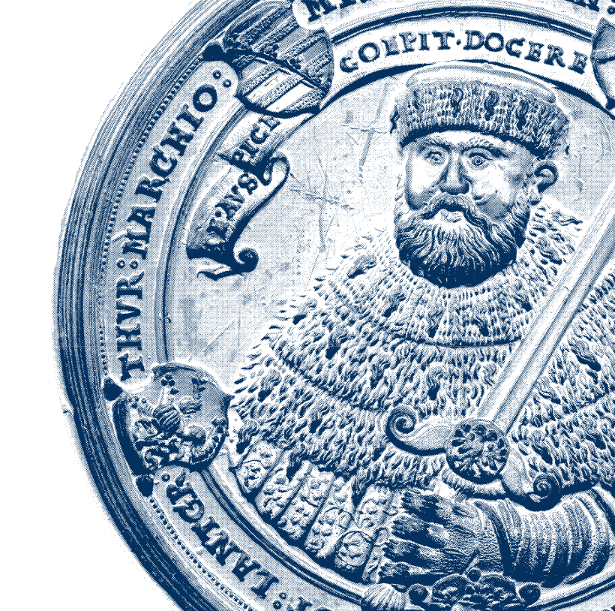
\includegraphics[width=1.0\textwidth]{pics/Hanfried}}

\begin{document}
\begin{frame}
 \titlepage
\end{frame}

\begin{frame}
\frametitle{Idee - Warum Musikempfehlungen + Big Data}
\begin{itemize}
 \item Music Streaming Services - Datenmengen wachsen
 \begin{itemize}
  \item Amazon Prime Music: 2 Millionen 
  \item Spotify: 35 Millionen
  \item Soundcloud+: 150 Millionen 
 \end{itemize}
\end{itemize}
\end{frame}

\begin{frame}
	\frametitle{Gibt es das nicht schon?}
	\begin{itemize}
		\item "Collaborative Filtering"
		\begin{itemize}
			\item ...
		\end{itemize}
		\item Forschung
		\begin{itemize}
			\item Viele Einzelaspekte separat beleuchtet (Meldodie, Rhythmus oder Klangfarbe)
		\end{itemize}
		\item Was fehlt?
		\begin{itemize}
			\item Parametrisierbare Empfehlungen (Schwerpunkte legen)
		\end{itemize}
	\end{itemize}
\end{frame}

\begin{frame}
	\frametitle{Datenextraktion Roadmap}
	\begin{itemize}
		\item Aufgaben\\
		\begin{minipage}[b]{0.85\linewidth}
			\centering
			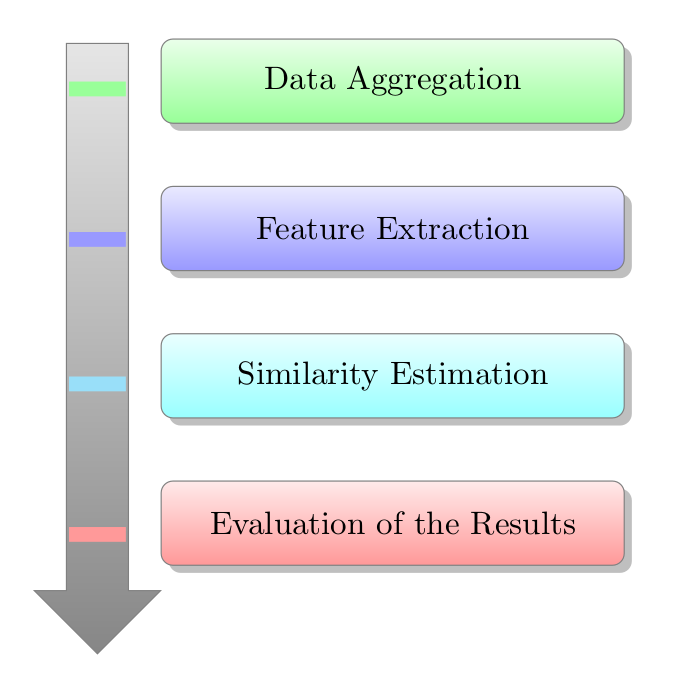
\includegraphics[width=0.7\textwidth]{pics/Org/Tasks.png}	
		\end{minipage}
	\end{itemize}
\end{frame}

\begin{frame}
	\frametitle{Daten}
	\begin{itemize}
		\item Free Music Archive - ca. 103.000 Lieder 
		\begin{itemize}
			\item Soundbeispiel
		\end{itemize}
		\item Private Musiksammlung - ca. 8000 Lieder
		\item 1517 Artists Dataset - 3180 Lieder
		\item Covers80 - 164 Lieder
		\item Summe: 1TB - ca 114000 verwertbare Songs 
	\end{itemize}
\end{frame}

\begin{frame}
	\frametitle{Datenextraktion Roadmap}
	\begin{itemize}
		\item Data Aggregation - Check\\
		\begin{minipage}[b]{0.85\linewidth}
			\centering
			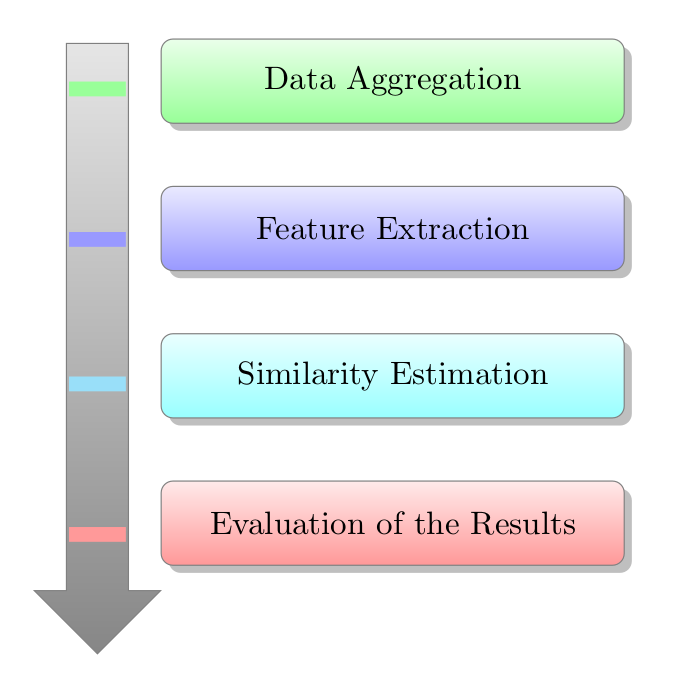
\includegraphics[width=0.7\textwidth]{pics/Org/Tasks.png}	
		\end{minipage}
	\end{itemize}
\end{frame}

\begin{frame}
	\frametitle{Feature Extraction Roadmap}
	\begin{itemize}
		\item Verschiedene Features parallel auf dem ARA-Cluster aus den Daten extrahieren:
			\begin{itemize}
			\item Melodie
			\begin{itemize}
				\item Noten
				\item Chromagramm
			\end{itemize}
			\item Rhythmus
			\begin{itemize}
				\item Beat Histogram 
				\item Rhythm Histrogram 
				\item Rhythm Pattern 
			\end{itemize}
			\item Klangfarbe
			\begin{itemize}
				\item MFCCs
			\end{itemize}
		\end{itemize}
	\end{itemize}
\end{frame}

\begin{frame}
	\frametitle{Ideale Features?}
	\begin{itemize}
		\item Melody Extraction
		\begin{figure}[ht]
			\begin{minipage}[b]{0.45\linewidth}
				\centering
				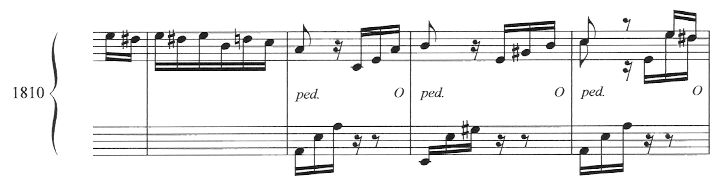
\includegraphics[width=\textwidth]{pics/Notes/felise.png}
				\caption{Für Elise~\cite{fe1}}
				\label{fe}
			\end{minipage}
			\hspace{0.5cm}
			\begin{minipage}[b]{0.45\linewidth}
				\centering
				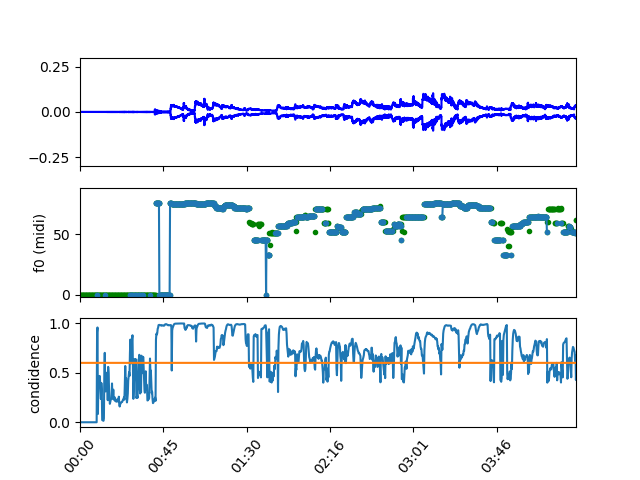
\includegraphics[width=\textwidth]{pics/Notes/feliseaubio.png}
				\caption{Pitch (Aubio)}
				\label{fep}
			\end{minipage}
		\end{figure}
	\end{itemize}
\end{frame}

\begin{frame}
	\frametitle{Nicht ganz so ideale Features}
	\begin{itemize}
		\item MIDI Noten aus Pitch vs. Original 
		\begin{figure}[ht]
			\begin{minipage}[b]{0.45\linewidth}
				\centering
				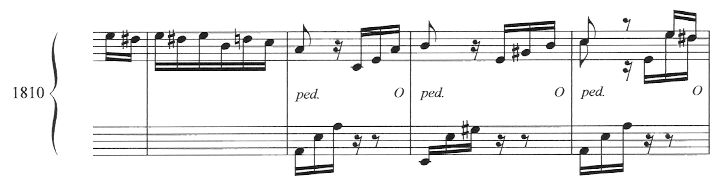
\includegraphics[width=\textwidth]{pics/Notes/felise.png}
				\caption{Für Elise~\cite{fe1}}
				\label{fe2}
			\end{minipage}
			\hspace{0.5cm}
			\begin{minipage}[b]{0.45\linewidth}
				\centering
				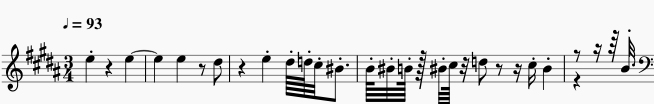
\includegraphics[width=\textwidth]{pics/Notes/feam.png}
				\caption{Erkannte Melodie (Aubio)}
				\label{fem}
			\end{minipage}
		\end{figure}
		\item \href{run:sounds/elise.mp3}{Play: Original}
		\item \href{run:sounds/Felise1.mp3}{Play: Noten}
		\item \href{run:sounds/Felise2.mp3}{Play: Erkannt}
	\end{itemize}
\end{frame}

\begin{frame}
	\frametitle{Klangfarbe}
	\begin{itemize}
		\item E-Gitarre (verzerrt) vs. Klavier
		\begin{figure}[ht]
			\begin{minipage}[b]{0.46\linewidth}
				\centering
				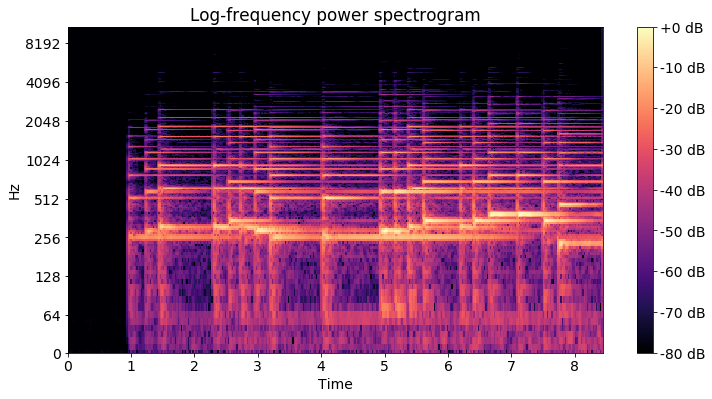
\includegraphics[width=\textwidth]{pics/MFCC/timbre_piano.png}
				\caption{Klavier}
				\label{piano}
			\end{minipage}
			\hspace{0.1cm}
			\begin{minipage}[b]{0.46\linewidth}
				\centering
				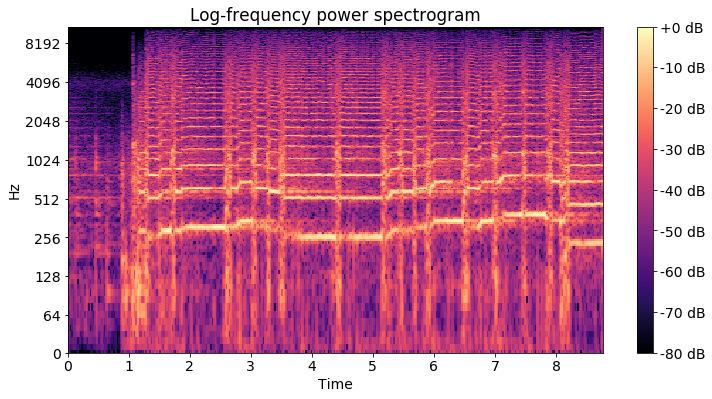
\includegraphics[width=\textwidth]{pics/MFCC/timbre_eguitar.png}
				\caption{Gitarre}
				\label{guit}
			\end{minipage}
			\hspace{0.1cm}
		\end{figure}	
		\item \href{run:sounds/piano.mp3}{Play: Klavier}
		\item \href{run:sounds/eguitar.mp3}{Play: Gitarre}
	\end{itemize}
\end{frame}

\begin{frame}
	\frametitle{Melodie Bandpass}
	\begin{itemize}
		\item 128 Hz bis 4096 Hz
		\begin{figure}[ht]
			\begin{minipage}[b]{0.46\linewidth}
				\centering
				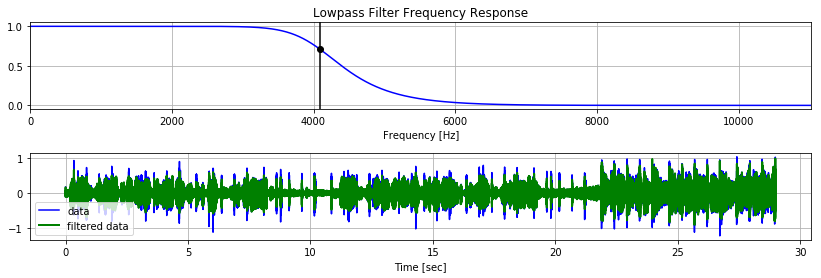
\includegraphics[width=\textwidth]{pics/Chroma/sialp.png}
				\caption{Tiefpass 128 Hz}
				\label{lp}
			\end{minipage}
			\hspace{0.1cm}
			\begin{minipage}[b]{0.46\linewidth}
				\centering
				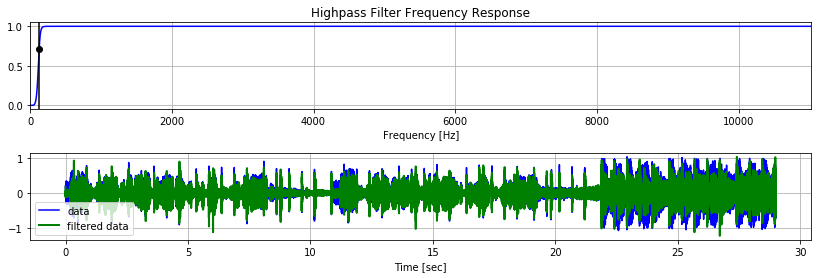
\includegraphics[width=\textwidth]{pics/Chroma/siahp.png}
				\caption{Hochpass 4096 Hz}
				\label{hp}
			\end{minipage}
			\hspace{0.1cm}
		\end{figure}	
		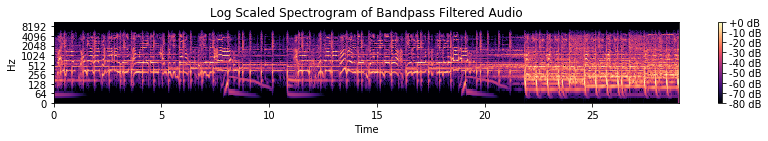
\includegraphics[width=0.8\textwidth]{pics/Chroma/siafft.png}
	\end{itemize}
\end{frame}

\begin{frame}
	\frametitle{Melodieextraktion}
	\begin{itemize}
		\item Noten aus Chromagramm (Oberwellen minimieren)
		\begin{figure}[ht]
			\begin{minipage}[b]{0.45\linewidth}
				\centering
				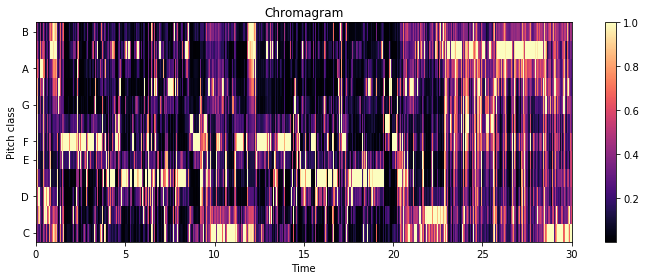
\includegraphics[width=\textwidth]{pics/Chroma/sia.png}
				\caption{Sia - Chandelier - Chromagramm}
				\label{sia}
			\end{minipage}
			\hspace{0.5cm}
			\begin{minipage}[b]{0.45\linewidth}
				\centering
				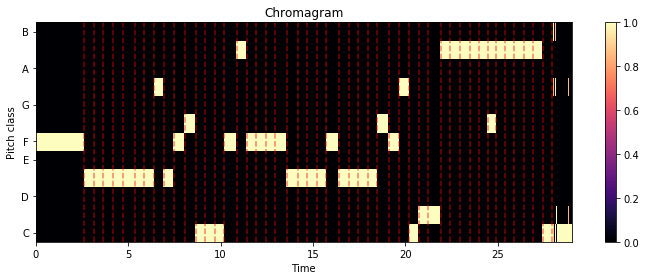
\includegraphics[width=\textwidth]{pics/Chroma/siafiltered.png}
				\caption{Sia - Chandelier - "Noten"}
				\label{siaf}
			\end{minipage}
		\end{figure}
		\item Noten zu String: [A, A, B, B, B, D, ... , D]
		\item Strings vergleichen (Levenshtein-Distanz) für Ähnlichkeitsschätzung 
	\end{itemize}
\end{frame}

\begin{frame}
	\frametitle{Kreuzkorrelation zwischen Chromagrammen}
	\begin{itemize}
		\item Kreuzkorrelation zwischen Matrix $X$ ($PxQ$ Matrix) und $Y$ ($MxN$ Matrix) zu Vektor C
			\begin{equation} \label{eq:conv1}
				C(l) = \sum_{m = 0}^{M - 1}{\sum_{n = 0}^{N - 1}{X(m, n)Y(m, n - l)}}
			\end{equation}
			\begin{equation} \label{eq:conv2}
				0 \leq l \leq N - Q
			\end{equation}
		\item Ergebnisvektor wird Hochpassgefiltert
	\end{itemize}
\end{frame}

\begin{frame}
	\frametitle{Kreuzkorrelation zwischen Chromagrammen}
	\begin{itemize}
		\item Zwei am Takt ausgerichtete Chromagramme
		\begin{figure}[ht]
			\begin{minipage}[b]{0.45\linewidth}
				\centering
				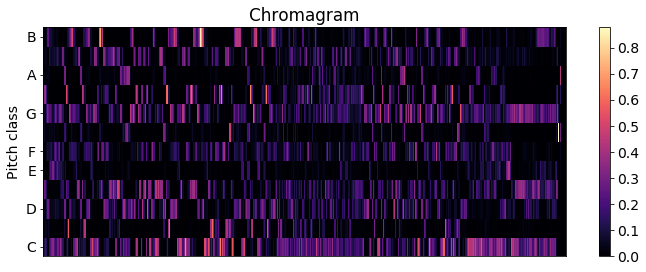
\includegraphics[width=\textwidth]{pics/Chroma/rach1chrom.png}
			\end{minipage}
			\hspace{0.5cm}
			\begin{minipage}[b]{0.45\linewidth}
				\centering
				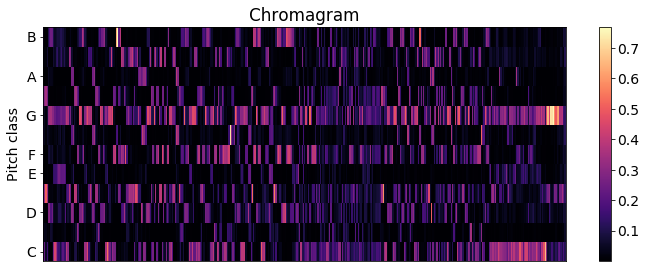
\includegraphics[width=\textwidth]{pics/Chroma/rach2chrom.png}
			\end{minipage}
		\end{figure}
		\item Ergebnisvektor (HP gefiltert;  Cover vs. verschiedene Lieder)
		\begin{figure}[ht]
			\begin{minipage}[b]{0.45\linewidth}
				\centering
				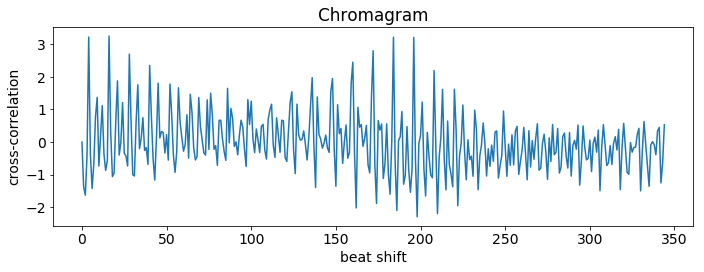
\includegraphics[width=\textwidth]{pics/Chroma/beatalignedchroma_corr_mean_filt.png}
			\end{minipage}
			\hspace{0.5cm}
			\begin{minipage}[b]{0.45\linewidth}
				\centering
				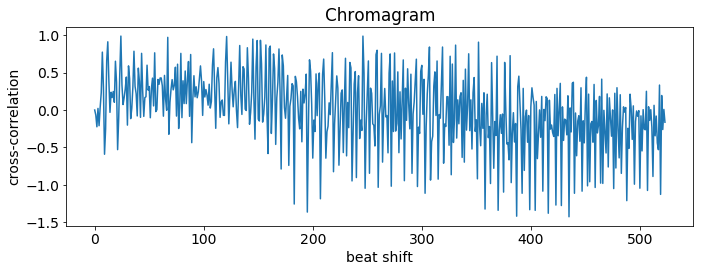
\includegraphics[width=\textwidth]{pics/Chroma/beatalignedchroma_corr_mean2_filt.png}
			\end{minipage}
		\end{figure}
	\end{itemize}
\end{frame}

\begin{frame}
	\frametitle{Und das waren nur die Melodiefeatures...}
	\begin{itemize}
		\item Rhythmus (z.B. Rhythm Patterns)
		\begin{minipage}[b]{0.9\linewidth}
			\centering
			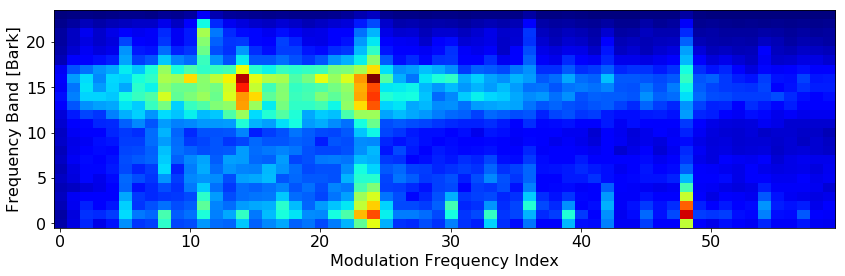
\includegraphics[width=0.9\textwidth]{pics/Beat/h_o_rp.png}
		\end{minipage}
		\item Klangfarbe/ Timbre (MFCCs)
		\begin{figure}[ht]
			\begin{minipage}[b]{0.375\linewidth}
				\centering
				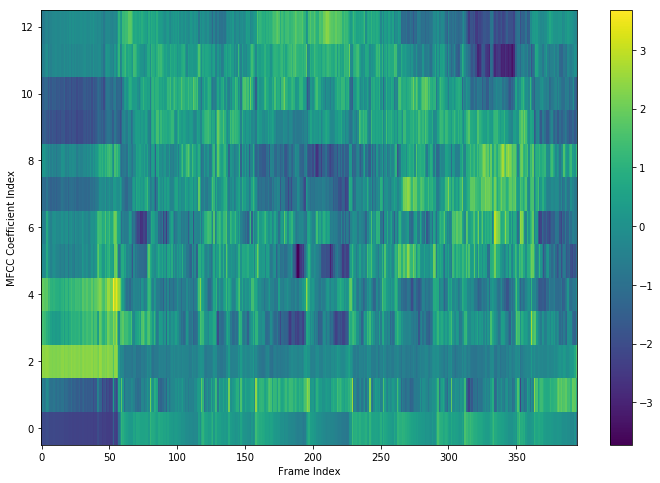
\includegraphics[width=\textwidth]{pics/MFCC/mfcc_guitar.png}
			\end{minipage}
			\hspace{0.5cm}
			\begin{minipage}[b]{0.375\linewidth}
				\centering
				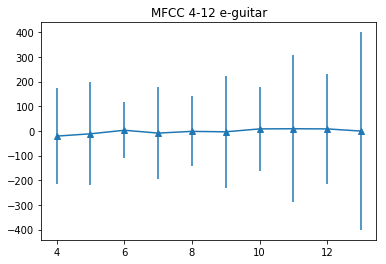
\includegraphics[width=\textwidth]{pics/MFCC/stat_eguitar.png}
			\end{minipage}
		\end{figure}
	\end{itemize}
\end{frame}

\begin{frame}
	\frametitle{Feature Extraction Timing}
	\begin{itemize}
		\item Feature Extraktion mit MPI4PY
		\begin{itemize}
			\item ca 5 min für 100 Lieder auf 4 CPU Cores 
			\begin{minipage}[b]{0.85\linewidth}
				\centering
				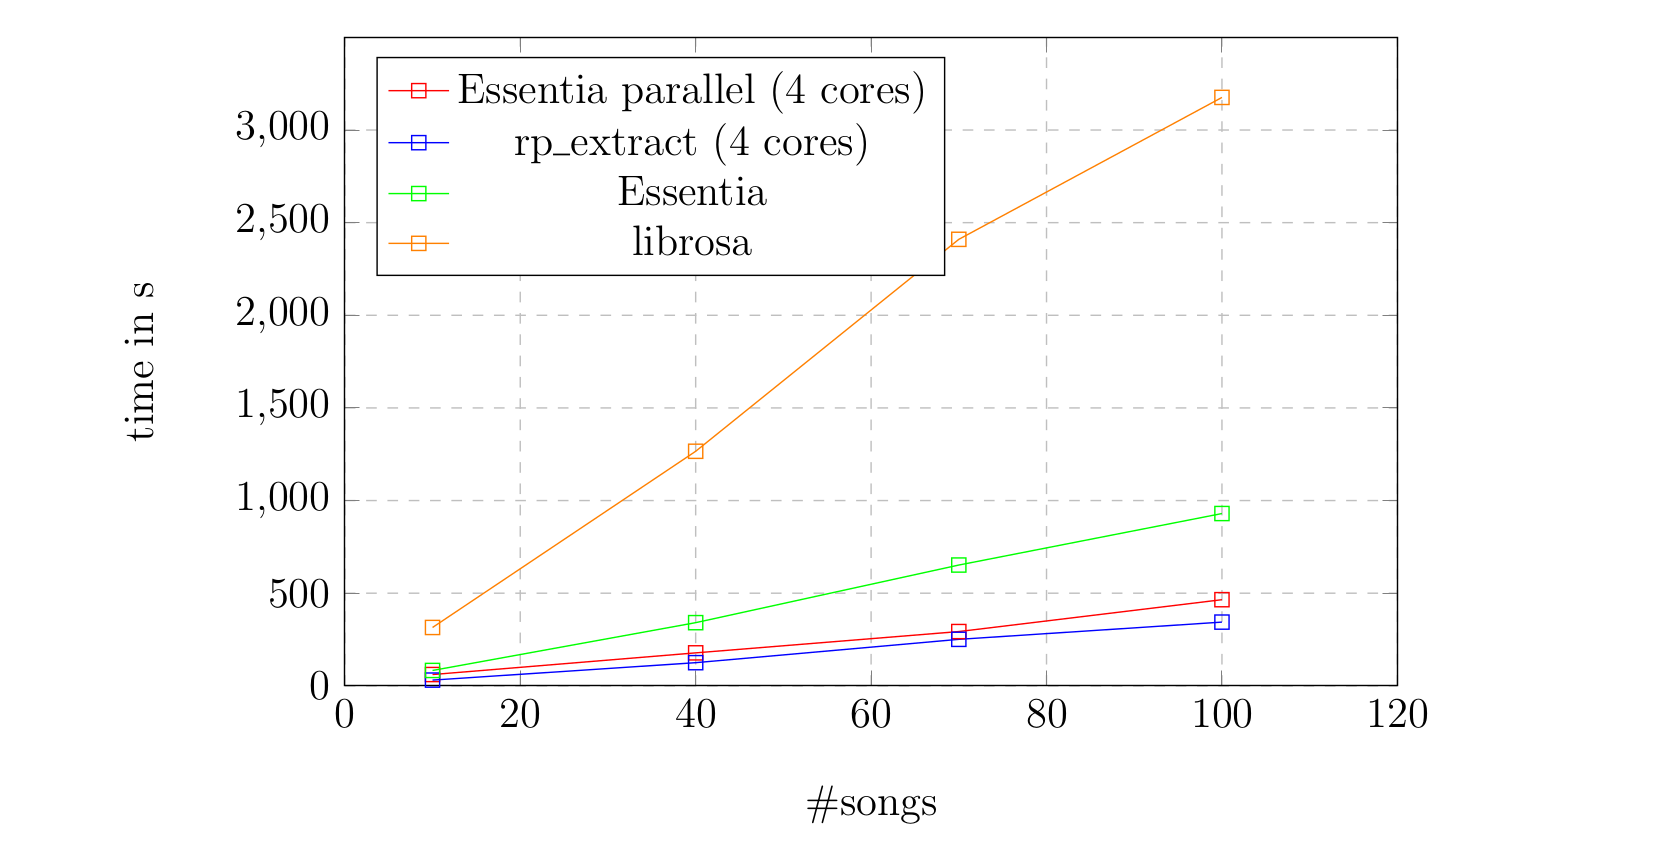
\includegraphics[width=0.95\textwidth]{pics/SparkFeat/featex.png}	
			\end{minipage}
			\item ca. 32,5 min für 102.000 Lieder auf 36 * 18 CPU Cores mit je 10GB RAM/Core
		\end{itemize}
	\end{itemize}
\end{frame}

\begin{frame}
	\frametitle{Übersicht}
	\begin{itemize}
		\item Feature Extraction - Check\\
		\begin{minipage}[b]{0.85\linewidth}
			\centering
			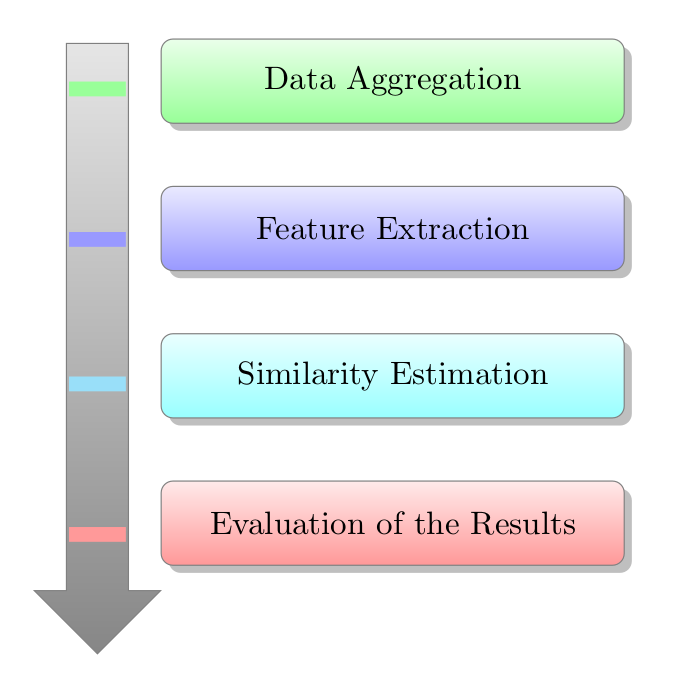
\includegraphics[width=0.7\textwidth]{pics/Org/Tasks.png}	
		\end{minipage}
	\end{itemize}
\end{frame}

\begin{frame}
	\frametitle{Ähnlichkeitsmaße}
	\begin{itemize}
		\item Melodie
		\begin{itemize}
			\item Levenshtein-Distanz zwischen zwei Strings
			\item Kreuzkorrelation zwischen zwei Chromagrammen 
		\end{itemize}
		\item Klangfarbe
		\begin{itemize}
			\item Jensen-Shannon Divergenz 
			\item Kullback-Leibler Divergenz
			\item Euklidischer Abstand 
		\end{itemize}
		\item Rhythmus
		\begin{itemize}
			\item Euklidischer Abstand (RP, RH, BH)
		\end{itemize}
	\end{itemize}
\end{frame}

\begin{frame}
	\frametitle{Big Data Framework}
	\begin{itemize}
		\item Apache Spark Cluster
		\begin{minipage}[b]{0.85\linewidth}
			\centering
			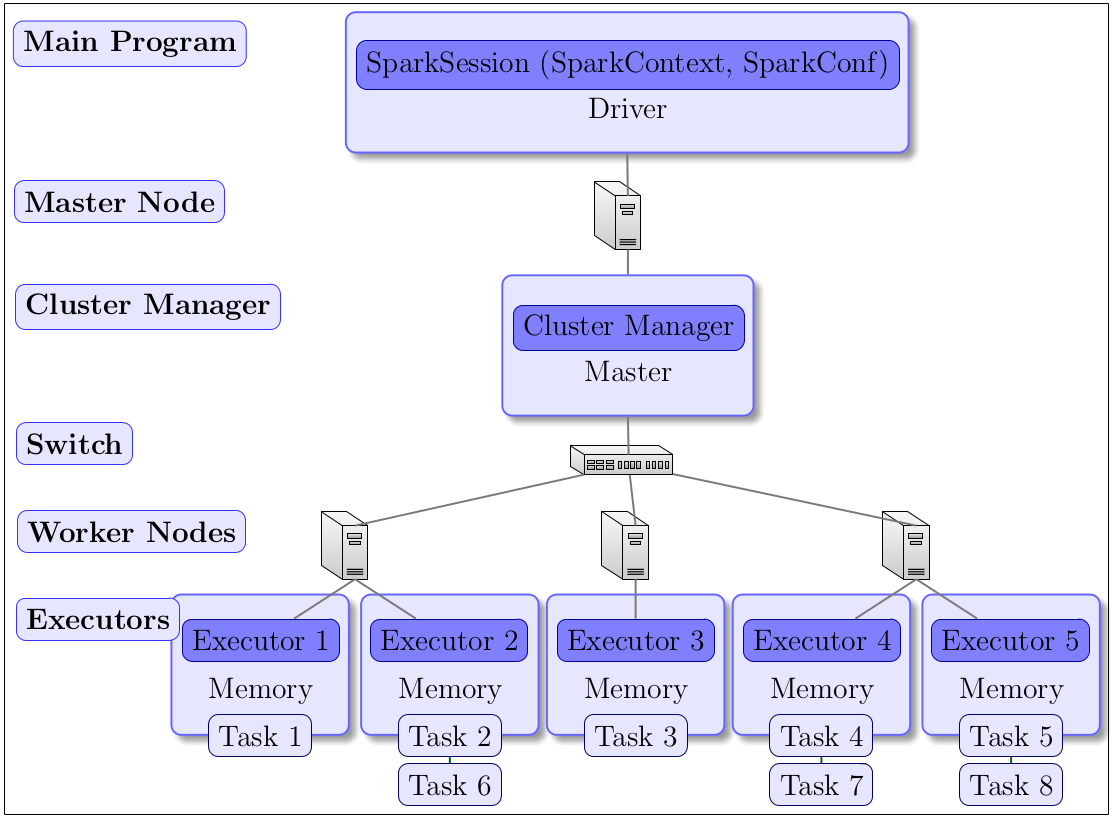
\includegraphics[width=0.95\textwidth]{pics/Spark/cluster.png}	
		\end{minipage}
	\end{itemize}
\end{frame}

\begin{frame}
	\frametitle{Ergebnisse}
	\begin{itemize}
		\item Ähnlichkeitsschätzung mit Spark
		\begin{itemize}
			\item 12 sec für 114.000 Lieder
			\begin{minipage}[b]{0.85\linewidth}
				\centering
				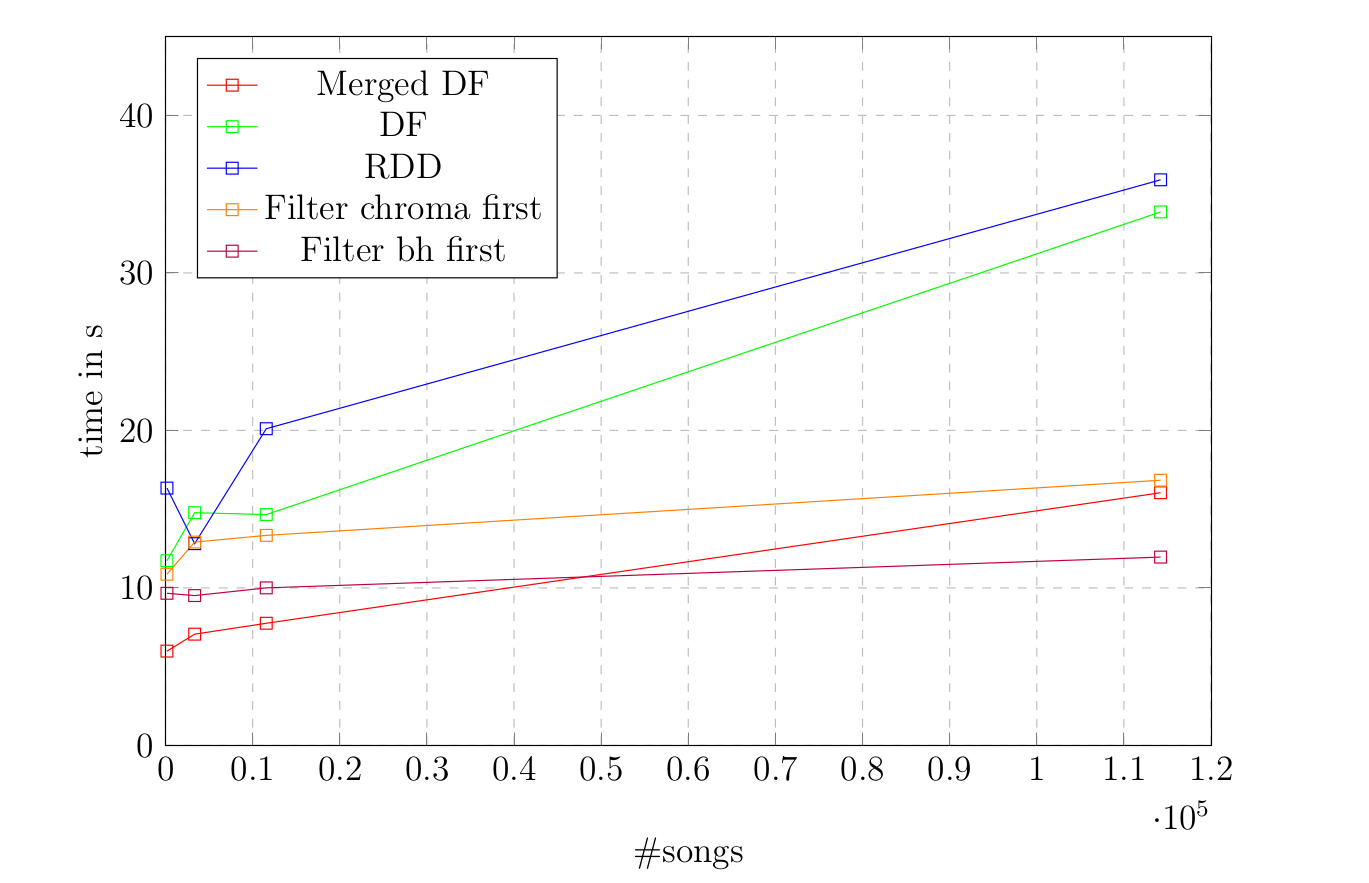
\includegraphics[width=0.95\textwidth]{pics/SparkFeat/simp.png}	
			\end{minipage}
		\end{itemize}
	\end{itemize}
\end{frame}

\begin{frame}
	\frametitle{Übersicht}
	\begin{itemize}
		\item Nächster Schritt: Evaluation\\
		\begin{minipage}[b]{0.85\linewidth}
			\centering
			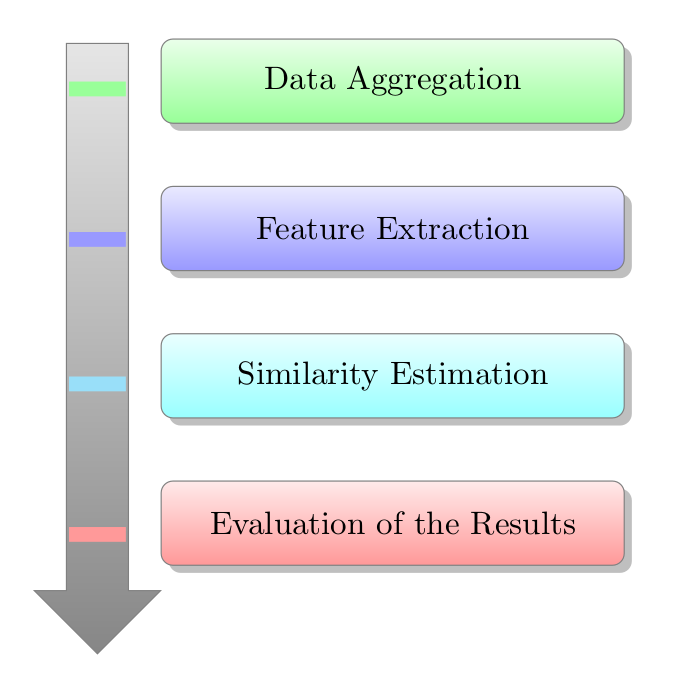
\includegraphics[width=0.7\textwidth]{pics/Org/Tasks.png}	
		\end{minipage}
	\end{itemize}
\end{frame}

\begin{frame}
	\frametitle{Korrelation der verschiedenen Distanzen}
	\begin{minipage}[b]{0.85\linewidth}
		\centering
		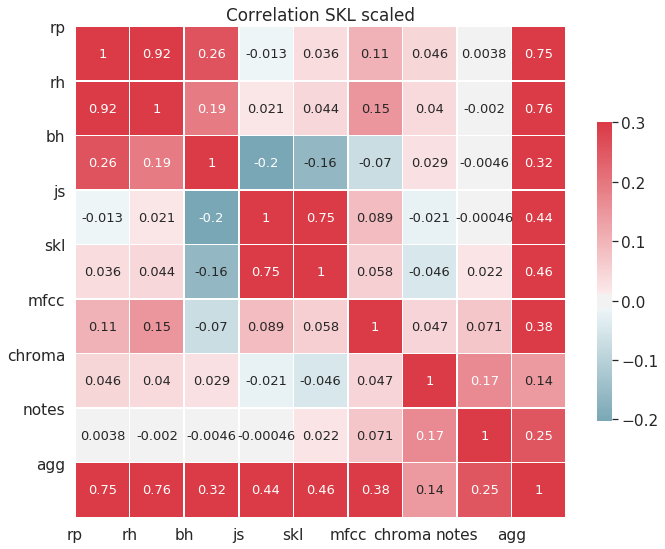
\includegraphics[width=0.7\textwidth]{pics/SparkFeat/skl_corr_scaled.png}	
	\end{minipage}
\end{frame}


\begin{frame}
	\frametitle{Genre Recall Rate}
	\begin{itemize}
		\item Empfehlungen für 10 Classical und 10 Rock/Pop Songs basierend auf Rhythmus- und Timbre-Features (3180 Testsongs)
		\begin{figure}[ht]
			\begin{minipage}[b]{0.47\linewidth}
				\centering
				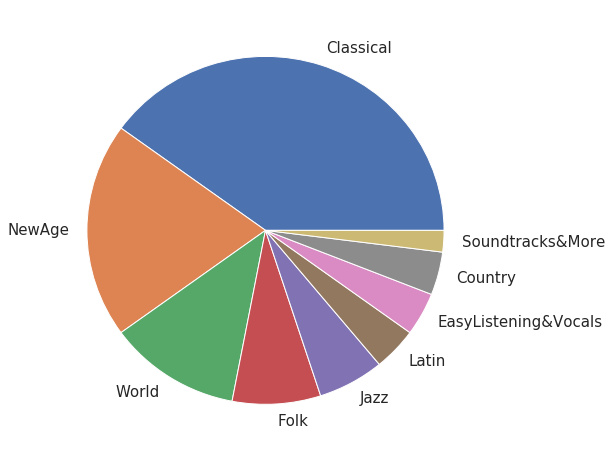
\includegraphics[width=\textwidth]{pics/SparkFeat/1517clasall.png}
			\end{minipage}
			\hspace{0.5cm}
			\begin{minipage}[b]{0.47\linewidth}
				\centering
				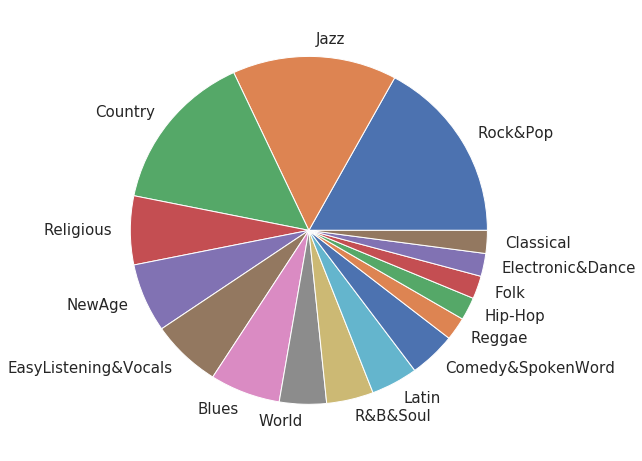
\includegraphics[width=\textwidth]{pics/SparkFeat/1517rockall.png}
			\end{minipage}
		\end{figure}
	\end{itemize}
\end{frame}

\begin{frame}
	\frametitle{Ergebnisse}
	\begin{itemize}
		\item Distanzen aller Lieder zu einem Electronic-Song (3180 Testsongs)
		\begin{minipage}[b]{0.75\linewidth}
			\centering
			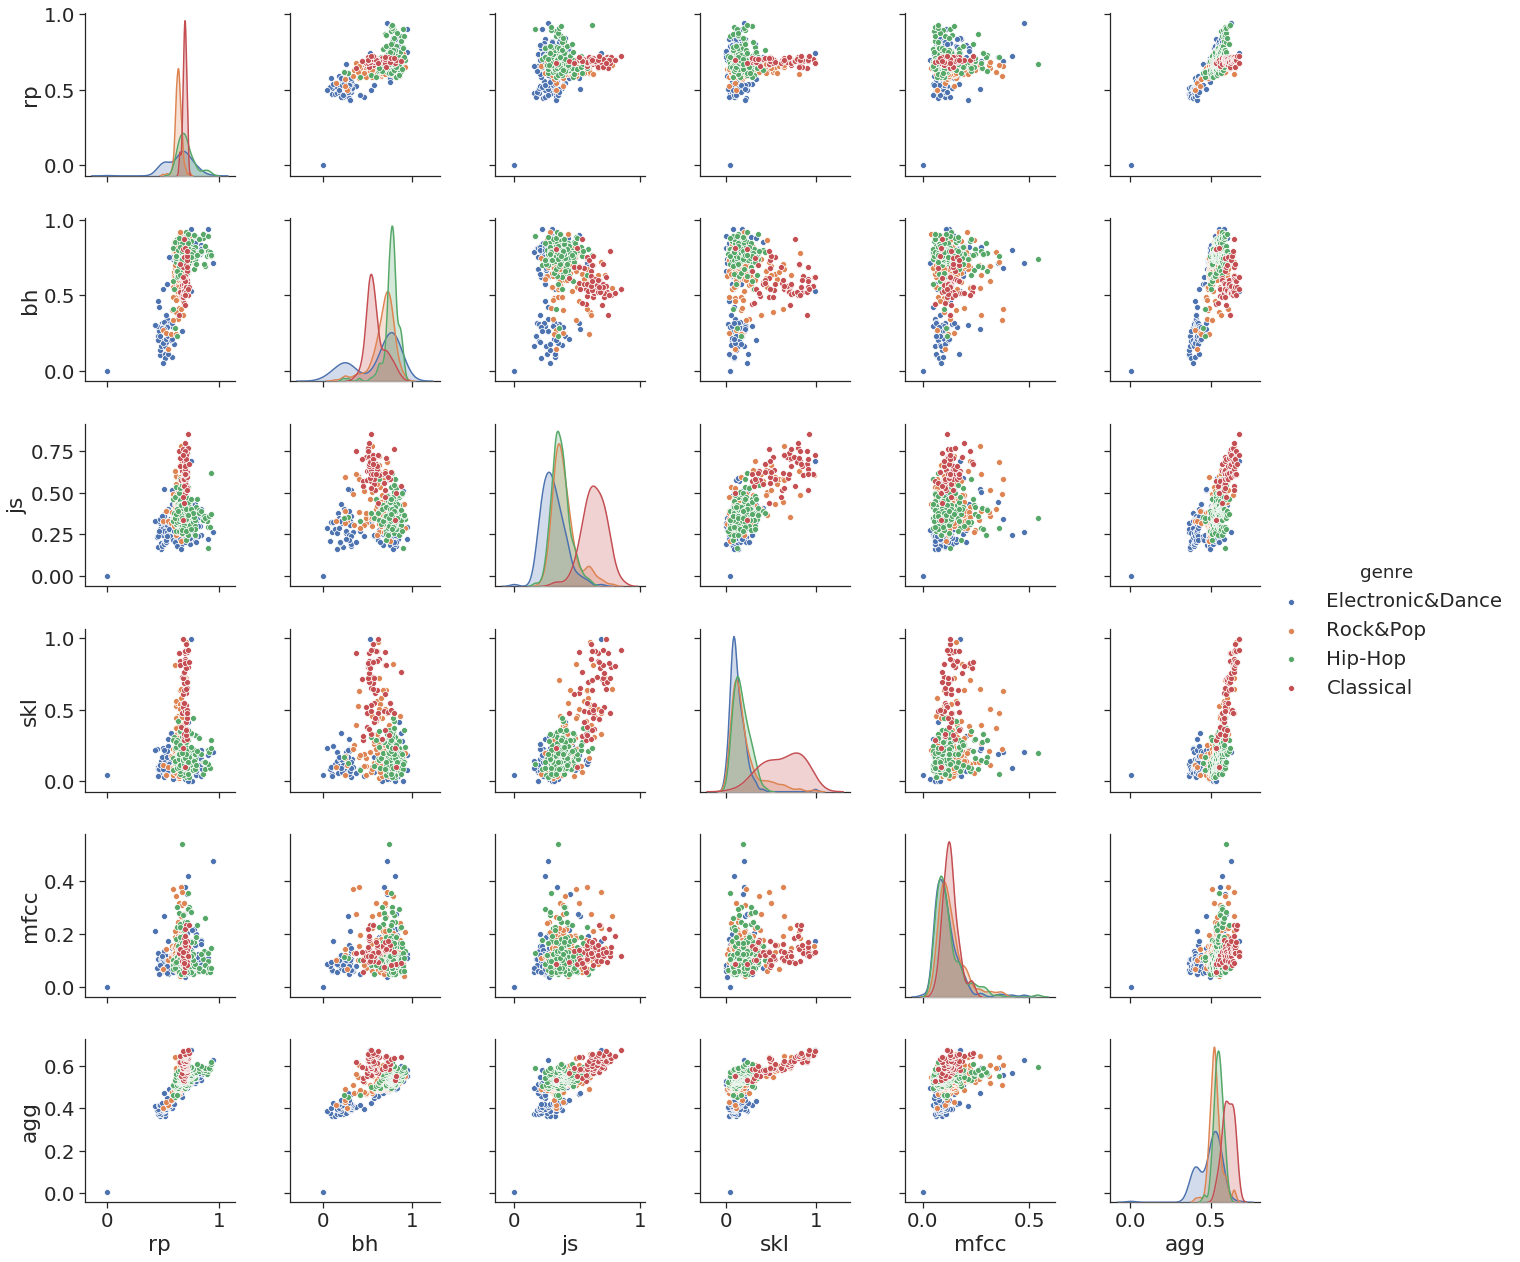
\includegraphics[width=0.95\textwidth]{pics/SparkFeat/electronic.png}	
		\end{minipage}
	\end{itemize}
\end{frame}

\begin{frame}
	\frametitle{Chroma Kreuzkorrelation - Top 6 Empfehlungen}
	\begin{itemize}
		\item Song request: 100 Meisterwerke der Klassik - Mozart - Alla Turca (Allegretto) (private
		collection)
		\begin{itemize}
			\item Mozart Collection / CD31 / KV331-3 Alla turca allegretto (private collection)
			\item Piano Collection / CD25 - Mozart - Alla Turca Allegretto (private collection)
			\item Piano Perlen / Mozart - Türkischer Marsch (private collection)
			\item FRITZ STEINEGGER - RONDO ALLA TURCA KV 331 (1517-Artists)
			\item 136071 (2Kutup - We Shall Cuddle Up And Sleep) (FMA dataset)
			\item Sean Bennett - Variations on the Turkish March (1517-Artists)
		\end{itemize}
	\end{itemize}
\end{frame}

\begin{frame}
	\frametitle{Cover Song Recognition Rate - covers80}
	\begin{minipage}[b]{0.75\linewidth}
		\centering
		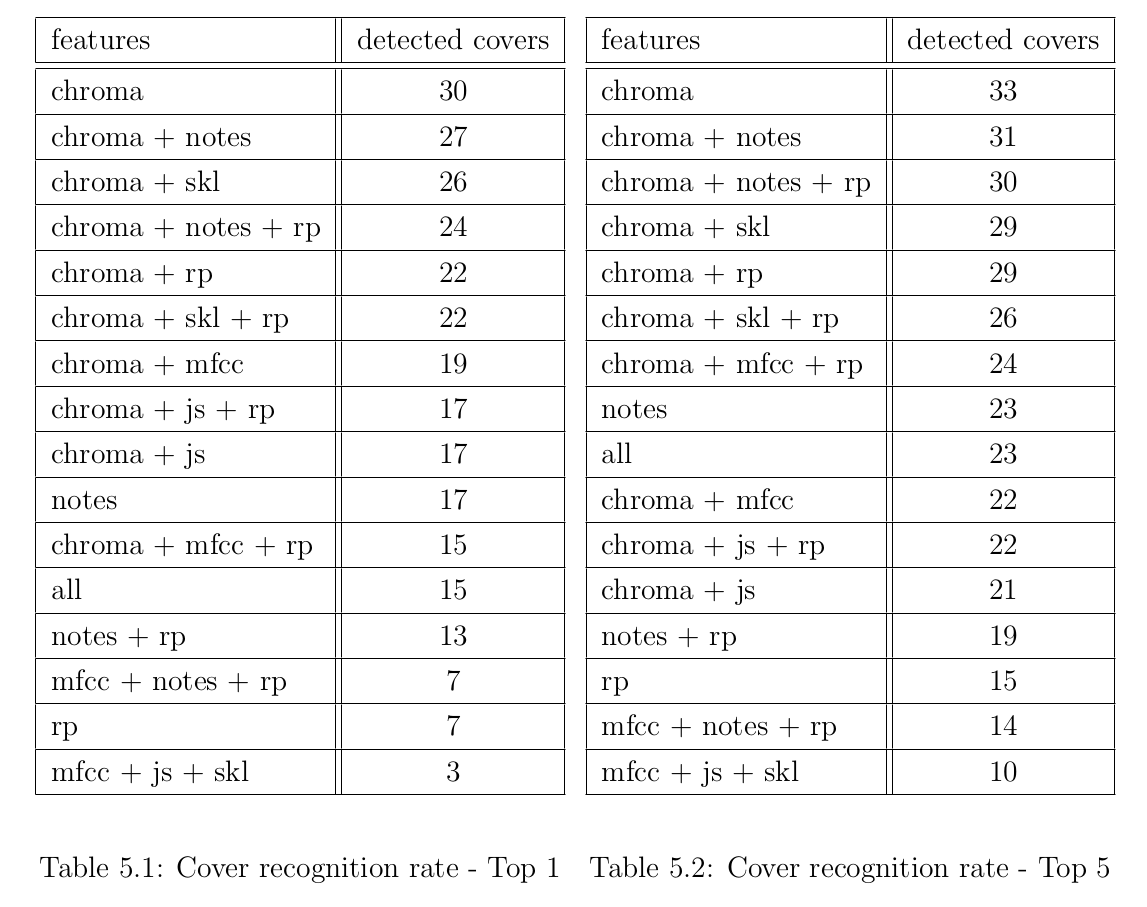
\includegraphics[width=0.95\textwidth]{pics/SparkFeat/covers.png}	
	\end{minipage}
\end{frame}

\begin{frame}
	\frametitle{Demonstration}
	\begin{itemize}
		\item Song Request 
		\begin{itemize}
			\item ...
		\end{itemize}
	\end{itemize}
\end{frame}

\begin{frame}
	\frametitle{Ausblick}
	\begin{itemize}
		\item MIREX 2020
		\begin{itemize}
			\item Paper?
		\end{itemize}
		\item Standalone Version?
		\item Bugfixes/ Erweiterungen (skalieren)/ Verbesserungen möglich - stehen in der Arbeit
	\end{itemize}
\end{frame}

\begin{frame}
	\frametitle{Quellen}
	\bibliographystyle{IEEEtran}
	\bibliography{literatur.bib}	
\end{frame}

\begin{frame}
	\frametitle{Danke für die Aufmerksamkeit}
	\begin{itemize}
		\item Fragen?
		\begin{itemize}
			\item ...
		\end{itemize}
	\end{itemize}
\end{frame}

\end{document}
